% cos k and sin k as functions on Z/8, repeated over two periods.
% Values are centred residues in {-3,...,3}.
\documentclass[tikz,border=8pt]{standalone}
\usepackage{amsmath,amssymb}
\begin{document}
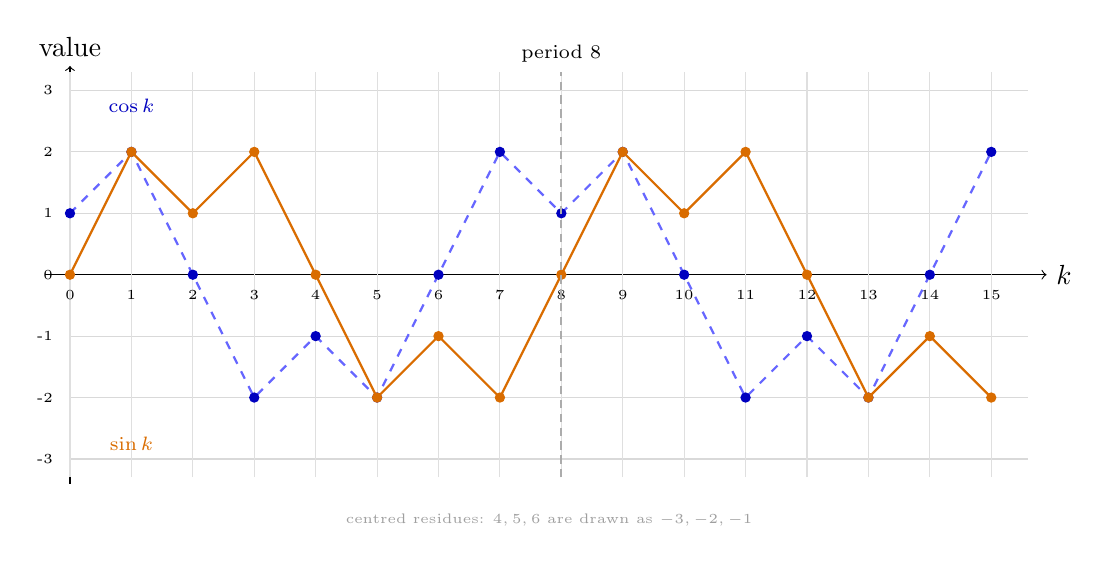
\begin{tikzpicture}[scale=0.78]
  % axes and grid
  \draw[->] (-0.4,0)--(15.9,0) node[right] {$k$};
  \draw[->] (0,-3.4)--(0,3.4) node[above] {value};
  \foreach \y in {-3,-2,-1,1,2,3} \draw[gray!30] (0,\y)--(15.6,\y);
  \foreach \k in {0,...,15} \draw[gray!25] (\k,-3.3)--(\k,3.3);
  \foreach \y in {-3,...,3} \node[font=\tiny,left] at (-0.12,\y) {\y};
  \foreach \k in {0,...,15} \node[font=\tiny,below] at (\k,-0.10) {\k};
  % cos k
  \draw[blue!60, dashed, line width=0.8pt]
    plot coordinates {(0,1)(1,2)(2,0)(3,-2)(4,-1)(5,-2)(6,0)(7,2)
                     (8,1)(9,2)(10,0)(11,-2)(12,-1)(13,-2)(14,0)(15,2)};
  \foreach \k/\v in {0/1,1/2,2/0,3/-2,4/-1,5/-2,6/0,7/2,
                     8/1,9/2,10/0,11/-2,12/-1,13/-2,14/0,15/2} {%
    \fill[blue!75!black] (\k,\v) circle (2.4pt);}
  % sin k
  \draw[orange!85!black, line width=0.8pt]
    plot coordinates {(0,0)(1,2)(2,1)(3,2)(4,0)(5,-2)(6,-1)(7,-2)
                     (8,0)(9,2)(10,1)(11,2)(12,0)(13,-2)(14,-1)(15,-2)};
  \foreach \k/\v in {0/0,1/2,2/1,3/2,4/0,5/-2,6/-1,7/-2,
                     8/0,9/2,10/1,11/2,12/0,13/-2,14/-1,15/-2} {%
    \fill[orange!85!black] (\k,\v) circle (2.4pt);}
  % period marker
  \draw[gray!65, densely dashed, line width=0.8pt] (8,-3.3)--(8,3.3);
  \node[font=\scriptsize,above] at (8,3.3) {period $8$};
  % legend
  \node[font=\scriptsize,text=blue!75!black] at (1.0,2.75) {$\cos k$};
  \node[font=\scriptsize,text=orange!85!black] at (1.0,-2.75) {$\sin k$};
  \node[font=\tiny,gray!75,align=center] at (7.8,-4.0)
    {centred residues: $4,5,6$ are drawn as $-3,-2,-1$};
\end{tikzpicture}
\end{document}
